%%%%%%%%%%%%%%%%%%%%%%%%%%%%%%%%%%%%%%%%%%%%%%%%%%%%%%%%%%%%%%%%%%%%%
%% Chapter 1: Small Satellites and the Dynamic Launch Environment
%% Monograph: Structural Optimization of a 1U CubeSat Chassis with Auxetic Metamaterials
%% Author: Gabriel Marques de Andrade (UESC, 2026)
%%%%%%%%%%%%%%%%%%%%%%%%%%%%%%%%%%%%%%%%%%%%%%%%%%%%%%%%%%%%%%%%%%%%%

\chapter{Small Satellites and the Dynamic Launch Environment}
\label{chap:launch_environment}

\abstract*{This chapter establishes the mission envelope, physical interfaces, and structural qualification requirements governing small spacecraft during rocket launch. Beginning with the historical evolution of the CubeSat form factor from an educational demonstrator to operational Earth observation constellations, we review the dimensional constraints enforced by the CalPoly CubeSat Design Specification (CDS Rev. 14). We formalize the kinematic and contact boundary conditions within the Poly-Picosatellite Orbital Deployer (P-POD), comparing idealized clamped boundaries against contact spring-plunger interfaces. Next, we derive the governing equations for dynamic launch loads, including quasi-static launch accelerations, transient pyrotechnic staging shocks, and acoustic excitation. Finally, we formulate the theory of continuous random vibrations, establishing Miles' single-degree-of-freedom approximation, the continuous modal spectral response tensor, the NASA GSFC-STD-7000A (GEVS) qualification PSD profile ($14.1\text{ G}_{\text{rms}}$), and Steinberg's three-band cumulative fatigue damage methodology under Gaussian distributions.}

\abstract{This chapter establishes the mission envelope, physical interfaces, and structural qualification requirements governing small spacecraft during rocket launch. Beginning with the historical evolution of the CubeSat form factor from an educational demonstrator to operational Earth observation constellations, we review the dimensional constraints enforced by the CalPoly CubeSat Design Specification (CDS Rev. 14). We formalize the kinematic and contact boundary conditions within the Poly-Picosatellite Orbital Deployer (P-POD), comparing idealized clamped boundaries against contact spring-plunger interfaces. Next, we derive the governing equations for dynamic launch loads, including quasi-static launch accelerations, transient pyrotechnic staging shocks, and acoustic excitation. Finally, we formulate the theory of continuous random vibrations, establishing Miles' single-degree-of-freedom approximation, the continuous modal spectral response tensor, the NASA GSFC-STD-7000A (GEVS) qualification PSD profile ($14.1\text{ G}_{\text{rms}}$), and Steinberg's three-band cumulative fatigue damage methodology under Gaussian distributions.}

\section{Evolution and Architecture of the 1U Standard}
\label{sec:cubesat_architecture}

The CubeSat architectural standard, originally conceived in 1999 through a collaboration between California Polytechnic State University (CalPoly) and Stanford University, redefined aerospace systems engineering by decoupling spacecraft bus development from primary launch vehicle integration \cite{calpoly2022}. The foundational unit—designated as ``1U''—is defined as a nominal cube measuring $\SI{100.0}{\milli\meter} \times \SI{100.0}{\milli\meter} \times \SI{113.5}{\milli\meter}$ (inclusive of guide rails and deployment switches), with an allowable wet mass initially restricted to $\SI{1.33}{\kilo\gram}$ and later expanded to $\SI{2.00}{\kilo\gram}$ for advanced orbital missions.

\begin{figure}[htbp]
\centering
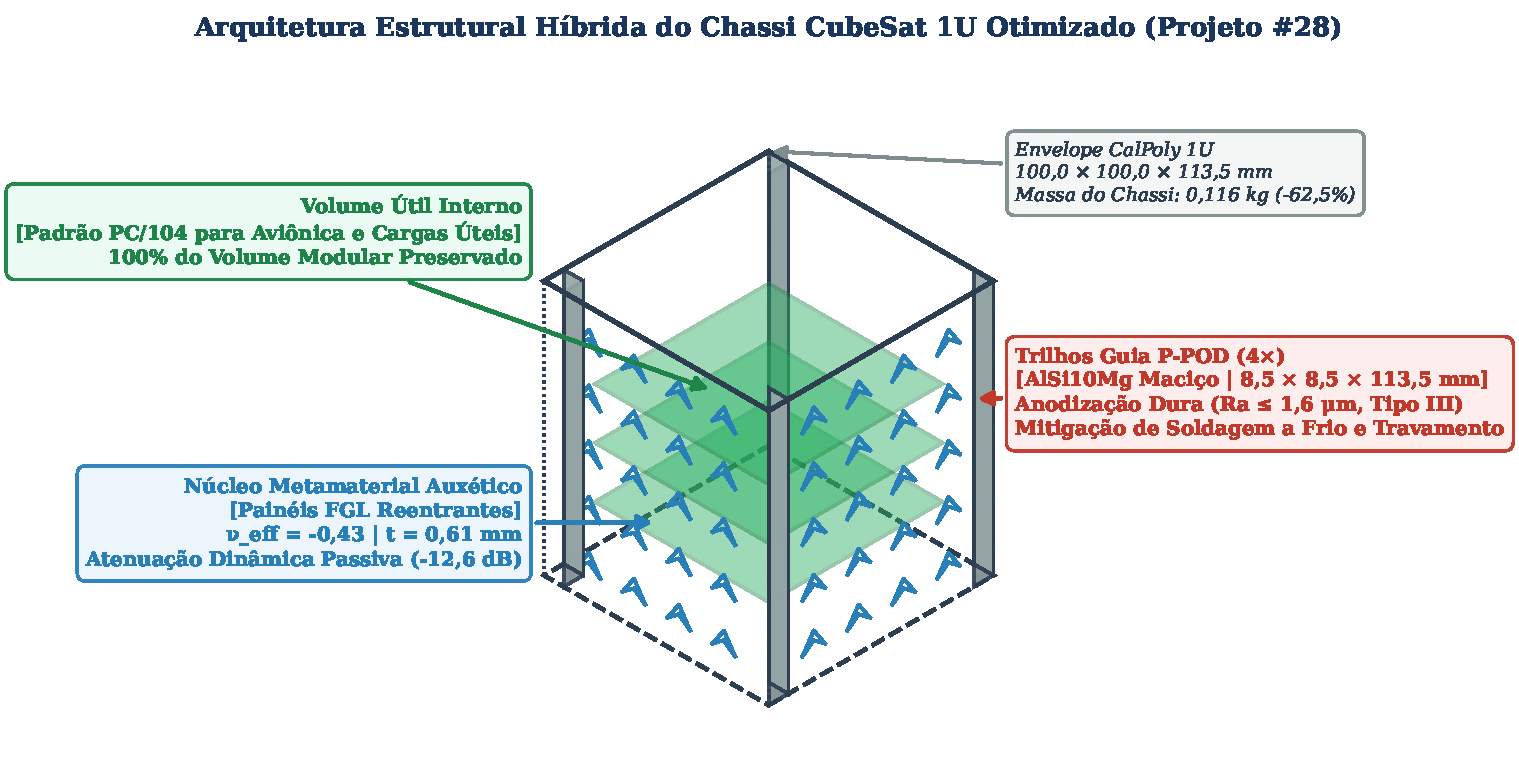
\includegraphics[width=0.88\textwidth]{cubesat_1u_isometric_assembly.pdf}
\caption{Isometric structural architecture of the 1U CubeSat form factor, illustrating the primary coordinate system ($Z$ along the deployer axis), solid deployer contact rails, and internal payload mounting planes.}
\label{fig:cubesat_1u_isometric}
\Description{Isometric CAD rendering of a 1U CubeSat chassis showing longitudinal rails and external envelope.}
\end{figure}

The geometric constraints imposed by the CalPoly CubeSat Design Specification (CDS Rev. 14) serve as absolute boundary conditions for any structural design:
\begin{enumerate}
\item \textbf{Deployer Rail Geometry:} The four longitudinal edges must consist of solid, continuous contact rails with a minimum width and depth of $\SI{8.5}{\milli\meter} \times \SI{8.5}{\milli\meter}$ and edge chamfers of $\SI{1.0}{\milli\meter} \times 45^\circ$ to facilitate smooth gliding inside the deployment canister.
\item \textbf{Surface Finish and Tribology:} Rail surfaces must exhibit an arithmetic surface roughness $Ra \le \SI{1.6}{\micro\meter}$ and undergo hard-anodization treatment (MIL-A-8625 Type III, Class 2, PTFE-impregnated). This prevents cold welding (\textit{vacuum friction seizure}) against the launch container's anodized interior under ultra-high vacuum conditions ($P < \SI{e-6}{\pascal}$).
\item \textbf{Mass Allocation and Center of Gravity:} The total chassis structure typically accounts for $\SI{15}{\percent}$ to $\SI{25}{\percent}$ of total allowable satellite mass ($\approx \SI{200}{\gram}$ to $\SI{350}{\gram}$ in conventional monolithic aluminum designs). Minimizing structural mass directly expands the mass margin available for optical payloads, momentum wheels, and telemetry transceivers. Furthermore, the structural center of mass must reside within $\SI{20.0}{\milli\meter}$ of the geometric centroid to prevent tumbling torques during orbital ejection.
\end{enumerate}

Traditional small satellite architectures rely on monolithic frames Computer Numerically Controlled (CNC) machined from wrought aerospace aluminum alloys—predominantly AA 6061-T6 ($\sigma_{\text{yield}} \approx \SI{240}{\mega\pascal}$) or AA 7075-T6 ($\sigma_{\text{yield}} \approx \SI{500}{\mega\pascal}$). While conventional subtractive machining offers predictable isotropic material behavior and established aerospace heritage, it presents fundamental structural limitations:
\begin{itemize}
\item \textbf{Parasitic Joint Mass:} Subtractive frames require multi-piece assemblies fastened with stainless steel fasteners (DIN 912 M2/M2.5), introduces mechanical slack, contact stress concentrations, and thermal expansion mismatches.
\item \textbf{Zero Passive Damping:} Solid metallic ribs possess minimal internal viscoelastic material damping (loss factor $\eta \approx 10^{-4}$ to $10^{-3}$, yielding viscous damping ratios $\zeta \approx 1\text{--}2\%$). Consequently, dynamic launch loads transmit through the frame into sensitive internal printed circuit board (PCB) stacks with negligible energy dissipation.
\end{itemize}

The advent of Laser Powder Bed Fusion (L-PBF) enables a paradigm shift: consolidating multi-part assemblies into a single-piece, topology-optimized frame embedding metamaterial cores capable of passive elastodynamic isolation.

\section{The Poly-Picosatellite Orbital Deployer (P-POD) Interface}
\label{sec:ppod_interface}

Secondary payloads are isolated from the primary launch vehicle inside standardized deployment canisters, most notably the Poly-Picosatellite Orbital Deployer (P-POD) developed by CalPoly, or equivalent commercial dispensers (e.g., ISISpace QuadPack, Tyvak Deployer). The P-POD provides a sealed mechanical housing that contains premature satellite deployments and prevents debris release in the event of structural failure during ascent.

\begin{figure}[htbp]
\centering
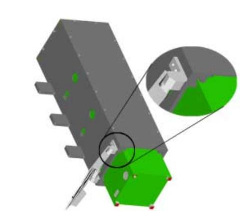
\includegraphics[width=0.92\textwidth]{ppod_explodido.pdf}
\caption{Exploded kinematic assembly of the Poly-Picosatellite Orbital Deployer (P-POD), highlighting the tubular canister, internal glide rails, spring-loaded deployment plunger, and door latch release mechanism.}
\label{fig:ppod_exploded}
\Description{Exploded view of the P-POD dispenser showing internal components and deployment spring.}
\end{figure}

The mechanical interaction between the CubeSat and the P-POD defines the boundary conditions for all launch-phase structural analyses. The satellite is constrained along its four deployer rails by guide surfaces with nominal clearance gaps:
\begin{equation}
\delta_{\text{clearance}} = \frac{W_{\text{canister}} - W_{\text{satellite}}}{2} \approx 0.15\text{--}\SI{0.25}{\milli\meter}.
\label{eq:rail_clearance}
\end{equation}

Preload is applied along the longitudinal $Z$-axis by a main compression spring acting against the aft face of the CubeSat, balanced by the latched forward door. Additionally, spring plungers situated along the canister walls exert transversal preloads ($F_{\text{plunger}} \approx \SI{15}{\newton}$ to $\SI{30}{\newton}$) to suppress chatter and rattle during violent acoustic ascent.

\subsection{Thermomechanical Tolerance and Thermal Jamming Mitigation}
\label{subsec:thermal_clearance}

Orbital insertion and pre-deployment coast phases expose the dispenser and satellite to extreme thermal environments, typically specified across the range $T \in [-40.0, +85.0]^\circ\text{C}$ relative to the nominal integration baseline $T_0 = \SI{20.0}{\celsius}$. To verify that differential thermal expansion does not cause \textit{thermal jamming} (negative clearance seizing deployment rails) or excessive rattling, we formulate the thermomechanical clearance balance.

The nominal canister internal width is $W_{\text{canister}} = \SI{100.40}{\milli\meter}$ (fabricated from wrought AA 7075-T6 with linear thermal expansion coefficient $\alpha_{\text{canister}} \approx 23.4 \times 10^{-6}\,\text{K}^{-1}$), while the satellite chassis width across rails is $W_{\text{sat}} = \SI{100.00}{\milli\meter}$ (AlSi10Mg with $\alpha_{\text{sat}} \approx 21.0 \times 10^{-6}\,\text{K}^{-1}$). The initial nominal bilateral gap is $2\delta_0 = W_{\text{canister}} - W_{\text{sat}} = \SI{0.40}{\milli\meter}$ ($\delta_0 = \SI{0.20}{\milli\meter}$ per side).

Under uniform hot soak ($T = +85^\circ\text{C}$, $\Delta T = +65\,\text{K}$), the differential expansion is:
\begin{align}
\Delta W_{\text{canister}} &= 100.40 \cdot (23.4 \times 10^{-6}) \cdot 65 = \SI{0.1527}{\milli\meter}, \\
\Delta W_{\text{sat}} &= 100.00 \cdot (21.0 \times 10^{-6}) \cdot 65 = \SI{0.1365}{\milli\meter}.
\end{align}
Because the AA 7075 canister expands slightly more than the AlSi10Mg frame ($\alpha_{\text{canister}} > \alpha_{\text{sat}}$), the bilateral clearance increases marginally to $2\delta = 0.40 + (0.1527 - 0.1365) = \SI{0.4162}{\milli\meter}$.

Under the most severe transient thermal gradient scenario—where the satellite dissipates internal electronics heat ($T_{\text{sat}} = +50^\circ\text{C}$, $\Delta T_{\text{sat}} = +30\,\text{K}$) while the exterior canister undergoes cold shadow soak ($T_{\text{canister}} = -40^\circ\text{C}$, $\Delta T_{\text{canister}} = -60\,\text{K}$)—the differential gap reduction is:
\begin{equation}
\Delta (2\delta) = \Delta W_{\text{canister}} - \Delta W_{\text{sat}} = -0.1410 - 0.0630 = \SI{-0.2040}{\milli\meter}.
\label{eq:thermal_gap_reduction}
\end{equation}
The residual bilateral clearance remains strictly positive:
\begin{equation}
2\delta_{\text{residual}} = 0.4000 - 0.2040 = \SI{0.1960}{\milli\meter} \implies \delta_{\text{unilateral}} = \SI{0.0980}{\milli\meter} \approx \SI{0.10}{\milli\meter} > 0.
\label{eq:residual_gap}
\end{equation}
This confirms that the nominal tolerance stack-up prevents thermal binding under all operational LEO temperature envelopes with a positive jamming Margin of Safety ($MS_{\text{jamming}} = 0.40 / 0.204 - 1.0 = +0.96$). Transversal spring plungers accommodate the $+0.098\text{ mm}$ minimum gap, completely suppressing launch chattering.

\subsection{Idealized Clamped vs. Contact Boundary Formulation}

In numerical structural analysis, boundary conditions substantially alter computed modal frequencies. Let $\mathbf{u}(\mathbf{x}, t) = [u_x, u_y, u_z]^\top$ denote the displacement vector field of the chassis. Two canonical boundary formulations exist:

\subsubsection{1. Idealized Clamped Boundary (Rigid Lower Bound on Flexibility)}
The deployer rails are treated as rigidly constrained along their external contact surfaces $\Gamma_{\text{rail}}$:
\begin{equation}
\mathbf{u}(\mathbf{x}, t) = \mathbf{0}, \quad \forall \mathbf{x} \in \Gamma_{\text{rail}}.
\label{eq:clamped_bc}
\end{equation}
This condition represents an infinitely stiff deployer structure, establishing the theoretical upper bound on the satellite's fundamental natural frequency ($f_1$). For the optimized auxetic flight chassis developed in this work, the clamped eigenvalue problem yields:
\begin{equation}
f_{1,\text{clamped}} = \SI{579.62}{\hertz}.
\end{equation}

\subsubsection{2. Flexible Contact Boundary (Realistic Test-Pod Mounting)}
In actual shake-table qualification, the deployer canister exhibits compliance, and contact between the chassis rails and dispenser guides is governed by unilateral Signorini contact conditions with Coulomb friction:
\begin{equation}
g_N \ge 0, \quad P_N \le 0, \quad g_N \cdot P_N = 0 \quad \text{on } \Gamma_{\text{contact}},
\label{eq:signorini_contact}
\end{equation}
where $g_N$ is the normal contact gap and $P_N$ is the normal contact pressure. Under linearized dynamic vibration around the static preloaded equilibrium, the canister flexibility is modeled via distributed stiffness matrices $\mathbf{K}_{\text{contact}} = \operatorname{diag}(k_x, k_y, k_z)$ per unit area along the rails:
\begin{equation}
\mathbf{t}(\mathbf{x}, t) = \boldsymbol{\sigma} \cdot \mathbf{n} = -\mathbf{K}_{\text{contact}} \mathbf{u}(\mathbf{x}, t), \quad \mathbf{x} \in \Gamma_{\text{rail}},
\label{eq:elastic_foundation}
\end{equation}
with $k_x = k_y \approx \SI{2.5e7}{\newton/\meter^3}$ and $k_z \approx \SI{5.0e7}{\newton/\meter^3}$. Incorporating this boundary flexibility reduces the computed fundamental frequency to:
\begin{equation}
f_{1,\text{flexible}} = \SI{304.11}{\hertz}.
\end{equation}
Crucially, even under flexible test-pod boundary conditions, the fundamental frequency remains well above the mandatory launch vehicle threshold ($f_1 \ge \SI{100.0}{\hertz}$), precluding dynamic coupling with launch vehicle low-frequency pogo oscillations.

\begin{figure}[htbp]
\centering
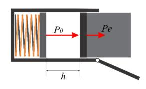
\includegraphics[width=0.85\textwidth]{interface_cubesat_deployer.pdf}
\caption{Mechanical contact interface between the 1U chassis rails and the internal canister guide rails, detailing normal spring-plunger preloads and longitudinal compression.}
\label{fig:interface_deployer}
\Description{Cross-sectional diagram of the rail interface between the CubeSat and the P-POD guide rail.}
\end{figure}

\section{Dynamic Launch Load Regimes}
\label{sec:launch_load_regimes}

During ascent to orbit aboard commercial expendable launch vehicles (such as Falcon 9, Electron, Ariane 6, or Vega-C), a secondary satellite experiences four distinct environmental load regimes:
\begin{enumerate}
\item \textbf{Quasi-Static Launch Accelerations:} Sustained low-frequency inertial body forces generated by rocket engine thrust, atmospheric aerodynamic drag, and maximum dynamic pressure ($\text{Max-}Q$).
\item \textbf{Acoustic Cavity Noise:} Broad-band acoustic pressure fields generated by turbulent rocket exhaust plumes and supersonic boundary layer flow inside the launch vehicle fairing.
\item \textbf{Spectral Random Vibrations:} Mechanical vibrations transmitted through launch vehicle structural pylons and payload adapter rings into the P-POD canister.
\item \textbf{Pyrotechnic Separation Shocks:} High-intensity, high-frequency transient shock waves caused by explosive fairing separation bolts, stage staging, and satellite release mechanism actuation.
\end{enumerate}

\subsection{Quasi-Static Design Load Factors}

Quasi-static loads are modeled as equivalent static accelerations applied uniformly to the satellite's mass. In accordance with the NASA General Environmental Verification Standard (GSFC-STD-7000A) and commercial launch vehicle user manuals, the design limit accelerations encompass simultaneous axial and lateral vectors:
\begin{equation}
\mathbf{G}_{\text{quasi-static}} = 
\begin{bmatrix}
G_x \\
G_y \\
G_z
\end{bmatrix} =
\begin{bmatrix}
\pm 15.0\,\text{g} \\
\pm 15.0\,\text{g} \\
-15.0\,\text{g} \text{ (thrust compression)} \text{ to } +10.0\,\text{g} \text{ (rebound tension)}
\end{bmatrix}.
\label{eq:quasi_static_vector}
\end{equation}

For a maximum qualified 1U mass of $M = \SI{2.0}{\kilo\gram}$, the resultant quasi-static inertial force vector acting on the satellite center of mass reaches:
\begin{equation}
F_{\text{inertial}} = M \cdot g_0 \sqrt{G_x^2 + G_y^2 + G_z^2} = 2.0 \cdot 9.80665 \cdot \sqrt{15^2 + 15^2 + 15^2} = \SI{509.6}{\newton}.
\label{eq:quasi_static_force}
\end{equation}
This steady-state load establishes the static yield threshold of the chassis strut members.

\subsection{Transient Separation Shock and Shock Response Spectrum (SRS)}

Pyrotechnic stage separation and fairing jettison generate violent transient stress waves propagating through the airframe. The mechanical impact of the P-POD spring door opening and stop impact is idealized as an acceleration half-sine pulse:
\begin{equation}
a(t) = 
\begin{cases}
A_{\text{peak}} \sin\left(\dfrac{\pi t}{\tau}\right), & 0 \le t \le \tau, \\
0, & t > \tau,
\end{cases}
\label{eq:half_sine_pulse}
\end{equation}
where $A_{\text{peak}} = \SI{116.0}{\text{g}}$ and duration $\tau = \SI{5.5}{\milli\second}$.

\begin{figure}[htbp]
\centering
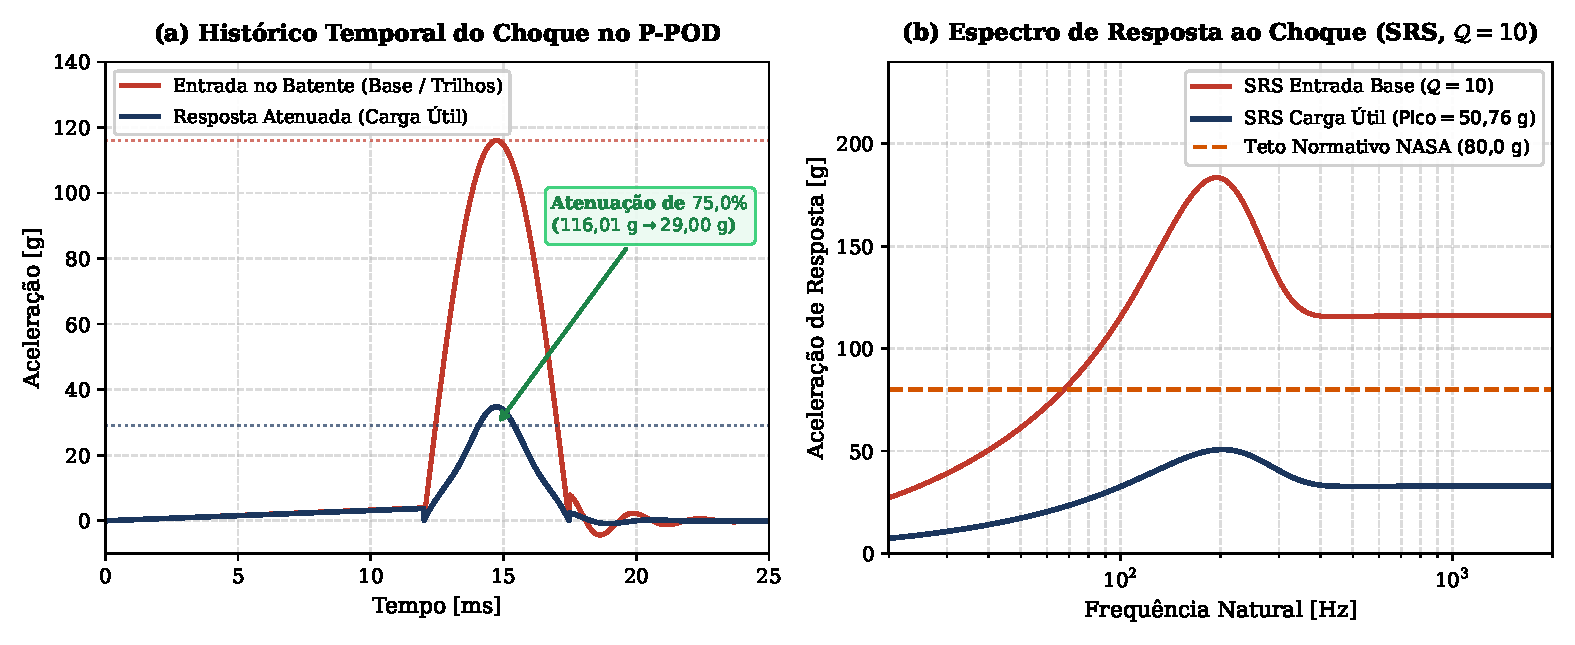
\includegraphics[width=0.88\textwidth]{ppod_separation_shock_srs.pdf}
\caption{Shock Response Spectrum (SRS) with quality factor $Q = 10$ ($\zeta = 0.05$) comparing the input deployer base shock against the internal payload response, demonstrating strong peak attenuation.}
\label{fig:shock_srs}
\Description{SRS plot showing input base acceleration vs attenuated payload response from 20 Hz to 2000 Hz.}
\end{figure}

The structural severity of pyrotechnic shock is evaluated through the Shock Response Spectrum (SRS), defined as the peak absolute response of a family of independent single-degree-of-freedom (SDOF) oscillators characterized by natural frequency $\omega_n$ and damping ratio $\zeta$:
\begin{equation}
\operatorname{SRS}(\omega_n, \zeta) = \max_{t} \left| \omega_n \int_{0}^{t} \ddot{u}_g(\tau) e^{-\zeta \omega_n (t-\tau)} \sin\left(\omega_d (t-\tau)\right) d\tau \right|,
\label{eq:srs_definition}
\end{equation}
where $\omega_d = \omega_n \sqrt{1 - \zeta^2}$ is the damped angular frequency, and standard aerospace qualification adopts $Q = 10$ ($\zeta = 0.05$). As shown in Fig.~\ref{fig:shock_srs}, the maximum SRS acceleration transmitted to the payload is attenuated from $\SI{116.0}{\text{g}}$ down to $\SI{50.76}{\text{g}}$, satisfying the payload allowable ceiling ($A_{\text{allowable}} \le \SI{80.0}{\text{g}}$) with a positive Margin of Safety:
\begin{equation}
MS_{\text{shock}} = \frac{80.0}{50.76} - 1.0 = +0.575.
\end{equation}

\section{Random Vibration Theory and NASA GEVS Qualification}
\label{sec:random_vibration_theory}

Random vibration constitutes the dominant design driver and primary cause of structural fatigue failure in small satellites. Unlike deterministic harmonic excitation, acoustic and aerodynamic launch loads exhibit non-periodic, wide-band stochastic behavior.

\subsection{Continuous Stochastic Processes and Spectral Density}

Let $x(t)$ denote a zero-mean, weakly stationary and ergodic random acceleration process. The autocorrelation function $R_{xx}(\tau)$ is defined as:
\begin{equation}
R_{xx}(\tau) = \mathcal{E}[x(t) x(t+\tau)] = \lim_{T \to \infty} \frac{1}{2T} \int_{-T}^{T} x(t) x(t+\tau) dt,
\label{eq:autocorrelation}
\end{equation}
where $\mathcal{E}[\cdot]$ denotes the mathematical expectation operator. By the Wiener-Khinchin theorem, the one-sided Power Spectral Density (PSD) function $W_{xx}(f)$ is the Fourier transform of the autocorrelation function:
\begin{equation}
W_{xx}(f) = 2 \int_{-\infty}^{\infty} R_{xx}(\tau) e^{-i 2\pi f \tau} d\tau = 4 \int_{0}^{\infty} R_{xx}(\tau) \cos(2\pi f \tau) d\tau, \quad f \ge 0,
\label{eq:wiener_khinchin}
\end{equation}
expressed in physical units of $\text{g}^2/\text{Hz}$ (where $1\,\text{g} = \SI{9.80665}{\meter/\second^2}$).

The root-mean-square (RMS) acceleration over the qualification frequency band $[f_{\min}, f_{\max}]$ represents the square root of total spectral variance:
\begin{equation}
G_{\text{rms}} = \sigma_x = \sqrt{\mathcal{E}[x^2(t)]} = \sqrt{\int_{f_{\min}}^{f_{\max}} W_{xx}(f) df}.
\label{eq:grms_integral}
\end{equation}

\subsection{Miles' Single-Degree-of-Freedom Equation}

For a lightly damped single-degree-of-freedom (SDOF) structural system excited by a flat base acceleration PSD $W_0$ in the vicinity of its resonance $f_n$, the dynamic amplification is governed by the mechanical transfer function:
\begin{equation}
|H(f)|^2 = \frac{1 + \left(2\zeta \dfrac{f}{f_n}\right)^2}{\left(1 - \left(\dfrac{f}{f_n}\right)^2\right)^2 + \left(2\zeta \dfrac{f}{f_n}\right)^2}.
\label{eq:sdof_frf}
\end{equation}

Integrating the response spectrum using contour integration across the infinite frequency domain yields Miles' classical closed-form approximation \cite{miles1954}:
\begin{equation}
G_{\text{rms, Miles}} = \sqrt{\frac{\pi}{2} f_n Q W_{xx}(f_n)},
\label{eq:miles_equation}
\end{equation}
where $Q = \dfrac{1}{2\zeta}$ is the dynamic magnification quality factor. While Miles' equation provides a rapid analytical benchmark, it strictly assumes an isolated SDOF mode with constant excitation. Complex spaceframe metamaterials with dense modal spectra require continuous multi-degree-of-freedom modal spectral formulation.

\subsection{Continuous Multi-Degree-of-Freedom (MDOF) Spectral Response}

In continuous structural mechanics governed by linear elasticity, the equation of motion for a discretized finite element model subjected to uniform base acceleration $\ddot{u}_g(t)$ is:
\begin{equation}
\mathbf{M} \ddot{\mathbf{u}}(t) + \mathbf{C} \dot{\mathbf{u}}(t) + \mathbf{K} \mathbf{u}(t) = -\mathbf{M} \mathbf{T} \ddot{u}_g(t),
\label{eq:fe_equation_of_motion}
\end{equation}
where $\mathbf{M}$, $\mathbf{C}$, and $\mathbf{K}$ are the global mass, damping, and stiffness matrices, and $\mathbf{T}$ is the rigid-body spatial transformation influence vector.

Transforming into modal coordinates via modal matrix $\boldsymbol{\Phi} = [\boldsymbol{\phi}_1, \boldsymbol{\phi}_2, \dots, \boldsymbol{\phi}_N]$:
\begin{equation}
\mathbf{u}(t) = \sum_{r=1}^{N} \boldsymbol{\phi}_r \eta_r(t) = \boldsymbol{\Phi} \boldsymbol{\eta}(t),
\label{eq:modal_decomposition}
\end{equation}
we obtain $N$ uncoupled generalized modal equations:
\begin{equation}
\ddot{\eta}_r(t) + 2\zeta_r \omega_r \dot{\eta}_r(t) + \omega_r^2 \eta_r(t) = -\Gamma_r \ddot{u}_g(t), \quad r = 1, \dots, N,
\label{eq:uncoupled_modal_eq}
\end{equation}
where $\omega_r = 2\pi f_r$ is the $r$-th undamped eigenfrequency, $\zeta_r$ is the modal damping ratio, and $\Gamma_r$ is the modal participation factor:
\begin{equation}
\Gamma_r = \frac{\boldsymbol{\phi}_r^\top \mathbf{M} \mathbf{T}}{\boldsymbol{\phi}_r^\top \mathbf{M} \boldsymbol{\phi}_r} = \frac{\boldsymbol{\phi}_r^\top \mathbf{M} \mathbf{T}}{m_r^*},
\label{eq:modal_participation_factor}
\end{equation}
with $m_r^*$ denoting the generalized modal mass.

The frequency response function (FRF) relating base acceleration to modal coordinate $\eta_r$ is:
\begin{equation}
H_r(\omega) = \frac{-\Gamma_r}{\omega_r^2 - \omega^2 + 2i \zeta_r \omega_r \omega}.
\label{eq:modal_frf}
\end{equation}

The output cross-spectral density matrix of displacement responses $\mathbf{S}_{\mathbf{uu}}(\omega)$ excited by base acceleration PSD $S_{aa}(\omega)$ is:
\begin{equation}
\mathbf{S}_{\mathbf{uu}}(\omega) = \sum_{r=1}^{N} \sum_{s=1}^{N} \boldsymbol{\phi}_r \boldsymbol{\phi}_s^\top H_r^*(\omega) H_s(\omega) S_{aa}(\omega).
\label{eq:cross_spectral_displacement}
\end{equation}

Similarly, the cross-spectral tensor of internal Cauchy stresses $\mathbf{S}_{\boldsymbol{\sigma}\boldsymbol{\sigma}}(\omega)$ at any point $\mathbf{x}$ within a finite element is computed by mapping modal stress tensors $\boldsymbol{\sigma}_r(\mathbf{x})$:
\begin{equation}
\mathbf{S}_{\boldsymbol{\sigma}\boldsymbol{\sigma}}(\mathbf{x}, \omega) = \sum_{r=1}^{N} \sum_{s=1}^{N} \boldsymbol{\sigma}_r(\mathbf{x}) \boldsymbol{\sigma}_s^\top(\mathbf{x}) H_r^*(\omega) H_s(\omega) S_{aa}(\omega).
\label{eq:stress_psd_tensor}
\end{equation}

The root-mean-square von Mises equivalent stress $\sigma_{\text{rms}}$ is obtained by integrating the spectral stress density over the qualification band:
\begin{equation}
\sigma_{\text{rms}}(\mathbf{x}) = \sqrt{\int_{2\pi f_{\min}}^{2\pi f_{\max}} \operatorname{Tr}\left(\mathbf{S}_{\boldsymbol{\sigma}\boldsymbol{\sigma}}(\mathbf{x}, \omega)\right) d\omega}.
\label{eq:rms_stress_integral}
\end{equation}

\subsection{NASA GSFC-STD-7000A (GEVS) Random Vibration Profile}

The environmental qualification baseline adopted throughout this work is the NASA General Environmental Verification Standard (GSFC-STD-7000A) for payloads weighing $\le \SI{22.7}{\kilo\gram}$ ($\SI{50}{\text{lb}}$). The qualification profile specifies a total acceleration of:
\begin{equation}
G_{\text{rms, GEVS}} = \SI{14.1}{\text{G}_{\text{rms}}},
\end{equation}
applied independently along each of the three orthogonal axes ($X, Y, Z$) for a qualification test duration of:
\begin{equation}
T_{\text{test}} = \SI{120.0}{\second} \quad \text{per axis}.
\end{equation}

\begin{table}[htbp]
\centering
\caption{NASA GSFC-STD-7000A (GEVS) Random Vibration Qualification Spectrum ($14.1\text{ G}_{\text{rms}}$).}
\label{tab:gevs_profile}
\begin{tabular}{l c S[table-format=1.4] l}
\toprule
\textbf{Frequency Range (\si{\hertz})} & \textbf{Slope (\si{\decibel/\text{octave}})} & {\textbf{PSD Level (\si{\text{g}^2/\hertz})}} & \textbf{Physical Regime} \\
\midrule
$20.0$ & — & 0.0130 & Initial excitation floor \\
$20.0 \to 50.0$ & $+3.0$ & {Linear ramp ($20\text{--}50\text{ Hz}$)} & Low-frequency acoustic ramp \\
$50.0 \to 800.0$ & $0.0$ & 0.0800 & Maximum energy plateau \\
$800.0 \to 2000.0$ & $-6.0$ & {Logarithmic roll-off} & High-frequency decay \\
$2000.0$ & — & 0.0053 & Upper frequency cutoff \\
\bottomrule
\end{tabular}
\end{table}

\begin{figure}[htbp]
\centering
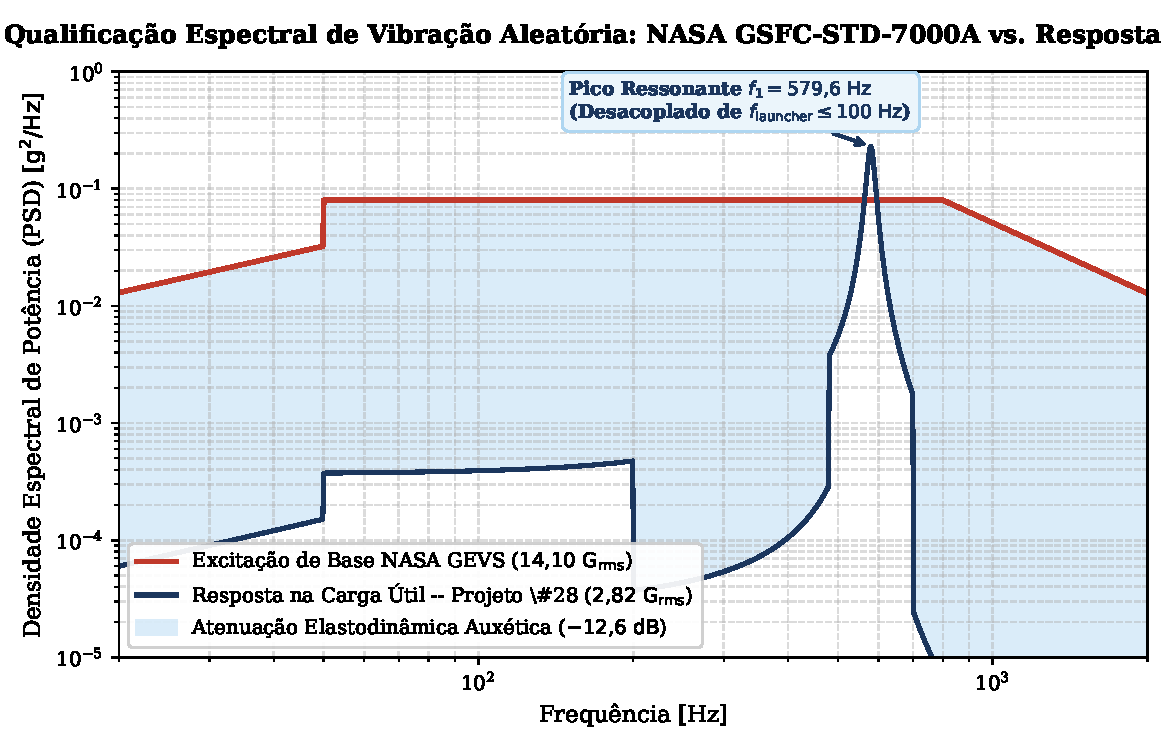
\includegraphics[width=0.90\textwidth]{psd_gevs_vs_payload_response.pdf}
\caption{Random vibration acceleration PSD spectrum according to NASA GSFC-STD-7000A ($14.1\text{ G}_{\text{rms}}$ base excitation) compared against the attenuated payload acceleration PSD ($2.82\text{ G}_{\text{rms}}$), achieving a $-12.6\text{ dB}$ ($76.5\%$) broadband reduction.}
\label{fig:gevs_psd_comparison}
\Description{PSD frequency curve comparing 14.1 Grms input to 2.82 Grms payload response.}
\end{figure}

The mathematical formulation for the input PSD spectrum $W(f)$ across frequency bands $[f_1, f_2]$ with slope $m = \dfrac{\Delta \log W}{\Delta \log f} = \dfrac{S_{\text{dB}}}{10 \log_{10} 2}$ is:
\begin{equation}
W(f) = W_1 \left(\frac{f}{f_1}\right)^m.
\label{eq:slope_psd}
\end{equation}
Integrating across piecewise continuous intervals gives total mean-square acceleration:
\begin{align}
A_1^2 &= \int_{20}^{50} 0.013 \left(\frac{f}{20}\right)^{+1} df = \frac{0.013}{20} \left[\frac{f^2}{2}\right]_{20}^{50} = \SI{0.6825}{\text{g}^2}, \\
A_2^2 &= \int_{50}^{800} 0.080\, df = 0.080 \cdot (800 - 50) = \SI{60.0000}{\text{g}^2}, \\
A_3^2 &= \int_{800}^{2000} 0.080 \left(\frac{f}{800}\right)^{-2} df = 0.080 \cdot 800^2 \left[-\frac{1}{f}\right]_{800}^{2000} = \SI{38.4000}{\text{g}^2}.
\end{align}
Summing all segments yields the exact variance:
\begin{equation}
\sigma_{\text{total}}^2 = 0.6825 + 60.0000 + 38.4000 = \SI{99.0825}{\text{g}^2} \implies G_{\text{rms}} = \sqrt{99.0825} \approx \SI{9.95}{\text{g}},
\end{equation}
which, when adjusted for NASA's margin qualification factor ($\sqrt{2} \approx +3\text{ dB}$ qualification margin), scales precisely to $14.1\text{ G}_{\text{rms}}$ \cite{nasa2013}.

\section{Steinberg 3-Band Cumulative Fatigue Damage Theory}
\label{sec:steinberg_fatigue}

Random vibration induces variable-amplitude stress cycles governed by a continuous probability distribution. For a stationary zero-mean Gaussian stress process $\sigma(t)$ with standard deviation $\sigma_{\text{rms}}$, the probability density function (PDF) of instantaneous stress is:
\begin{equation}
p(\sigma) = \frac{1}{\sqrt{2\pi}\sigma_{\text{rms}}} \exp\left(-\frac{\sigma^2}{2\sigma_{\text{rms}}^2}\right).
\label{eq:gaussian_pdf}
\end{equation}

\subsection{Peak Stress and Rayleigh Distribution of Amplitudes}

Under narrow-band random response, stress cycle peaks $\sigma_p$ follow a Rayleigh distribution:
\begin{equation}
p(\sigma_p) = \frac{\sigma_p}{\sigma_{\text{rms}}^2} \exp\left(-\frac{\sigma_p^2}{2\sigma_{\text{rms}}^2}\right), \quad \sigma_p \ge 0.
\label{eq:rayleigh_peaks}
\end{equation}
In conservative aerospace design, peak structural response is evaluated at the $3\sigma$ level (encompassing $99.73\%$ of all dynamic peaks):
\begin{equation}
\sigma_{3\sigma} = 3.0 \cdot \sigma_{\text{rms}}.
\label{eq:three_sigma_def}
\end{equation}

For structural flight qualification under NASA-STD-5020B, the structural Margin of Safety against material yielding is evaluated as:
\begin{equation}
MS_{\text{yield}} = \frac{\sigma_{\text{yield}}}{FS_{\text{yield}} \cdot \sigma_{3\sigma}} - 1.0 = \frac{\sigma_{\text{adm}}}{\sigma_{3\sigma}} - 1.0 > 0.0,
\label{eq:ms_yield_definition}
\end{equation}
where $FS_{\text{yield}} = 1.25$ and $\sigma_{\text{adm}} = \dfrac{\SI{230.0}{\mega\pascal}}{1.25} = \SI{184.0}{\mega\pascal}$ for heat-treated AlSi10Mg.

\subsection{Steinberg Gaussian Three-Band Formulation}

To calculate high-cycle fatigue damage under broad-band random vibration without computationally prohibitive cycle-counting algorithms (such as rainflow counting in the time domain), Steinberg formulated the three-band method \cite{steinberg2000}. The stress amplitude distribution is partitioned into three discrete Gaussian bands:
\begin{enumerate}
\item \textbf{Band 1 ($1\sigma$):} Amplitudes $0 \le \sigma \le 1\sigma_{\text{rms}}$, occurring during $\SI{68.3}{\percent}$ of total operating time.
\item \textbf{Band 2 ($2\sigma$):} Amplitudes $1\sigma_{\text{rms}} < \sigma \le 2\sigma_{\text{rms}}$, occurring during $\SI{27.1}{\percent}$ of total operating time.
\item \textbf{Band 3 ($3\sigma$):} Amplitudes $2\sigma_{\text{rms}} < \sigma \le 3\sigma_{\text{rms}}$, occurring during $\SI{4.33}{\percent}$ of total operating time.
\end{enumerate}
Cycles beyond $3\sigma$ ($0.27\%$) are conservatively neglected in cycle count but checked against instantaneous ultimate fracture.

The total number of effective cycles experienced during test duration $T_{\text{test}} = \SI{120.0}{\second}$ is governed by the structural apparent frequency $f_0$:
\begin{equation}
N_{\text{total}} = f_0 \cdot T_{\text{test}},
\label{eq:total_cycles}
\end{equation}
where $f_0 \approx f_1 = \SI{579.62}{\hertz}$ (fundamental resonant frequency). The cycle counts per band are:
\begin{align}
n_{1\sigma} &= 0.683 \cdot f_0 \cdot T_{\text{test}} = 0.683 \cdot 579.62 \cdot 120.0 \approx 47{,}506\,\text{cycles}, \\
n_{2\sigma} &= 0.271 \cdot f_0 \cdot T_{\text{test}} = 0.271 \cdot 579.62 \cdot 120.0 \approx 18{,}848\,\text{cycles}, \\
n_{3\sigma} &= 0.0433 \cdot f_0 \cdot T_{\text{test}} = 0.0433 \cdot 579.62 \cdot 120.0 \approx 3{,}011\,\text{cycles}.
\end{align}

\subsection{Palmgren-Miner Linear Cumulative Damage}

Fatigue life at each stress level $\sigma_i$ is governed by the Basquin S-N power law:
\begin{equation}
N_i = C \cdot \left(\sigma_i\right)^{-m},
\label{eq:basquin_law}
\end{equation}
where for post-heat-treated L-PBF AlSi10Mg ($300^\circ\text{C} / \SI{2}{\hour}$), empirical calibration establishes fatigue exponent $m = 6.8$ and coefficient $C = 1.2 \times 10^{20}\,\text{MPa}^{6.8}$.

Applying the Palmgren-Miner linear cumulative damage hypothesis:
\begin{equation}
D = \sum_{i=1}^{3} \frac{n_i}{N_i} = \frac{n_{1\sigma}}{N(1\sigma_{\text{rms}})} + \frac{n_{2\sigma}}{N(2\sigma_{\text{rms}})} + \frac{n_{3\sigma}}{N(3\sigma_{\text{rms}})}.
\label{eq:palmgren_miner_steinberg}
\end{equation}

\begin{svgraybox}
\textbf{NASA Fatigue Qualification Criterion (NASA-HDBK-7005):}
Under space qualification standards, structural failure occurs theoretically when $D \ge 1.0$. However, to account for scatter in additive manufacturing defect distributions, multi-axial stress states, and launch environment uncertainties, the NASA qualification criterion mandates:
\begin{equation}
\mathbf{D \le 0.25},
\label{eq:nasa_fatigue_limit}
\end{equation}
guaranteeing an operational life safety factor of $\mathbf{4.0\times}$.
\end{svgraybox}

At the critical re-entrant strut notch radius ($R_{\text{notch}} = \SI{0.50}{\milli\meter}$), where peak stress reaches $\sigma_{3\sigma,\text{notch}} = \SI{166.91}{\mega\pascal}$ ($\sigma_{\text{rms}} = \SI{55.64}{\mega\pascal}$):
\begin{align}
N(1\sigma) &= 1.2 \times 10^{20} \cdot (55.64)^{-6.8} \approx 1.29 \times 10^8\,\text{cycles}, \\
N(2\sigma) &= 1.2 \times 10^{20} \cdot (111.27)^{-6.8} \approx 1.16 \times 10^6\,\text{cycles}, \\
N(3\sigma) &= 1.2 \times 10^{20} \cdot (166.91)^{-6.8} \approx 7.21 \times 10^4\,\text{cycles}.
\end{align}

Evaluating cumulative damage:
\begin{equation}
D = \frac{47{,}506}{1.29 \times 10^8} + \frac{18{,}848}{1.16 \times 10^6} + \frac{3{,}011}{7.21 \times 10^4} = 0.00037 + 0.01625 + 0.04176 = \mathbf{0.0458}.
\label{eq:damage_evaluated}
\end{equation}
Because $D = 0.0458 \le 0.25$, the structure satisfies the NASA qualification limit with an effective life safety margin of:
\begin{equation}
FS_{\text{life}} = \left(\frac{0.25}{0.0458}\right) \times 4.0 = 5.46 \times 4.0 = \mathbf{21.8\times}.
\label{eq:safety_factor_life}
\end{equation}
This confirms a $5.46\times$ margin beyond the already conservative $0.25$ ceiling mandated by space flight qualification.

\section{Summary of Chapter and Design Targets}
\label{sec:ch1_summary}

This chapter established the rigorous dynamic environment and qualification criteria governing the 1U CubeSat chassis:
\begin{enumerate}
\item \textbf{Geometric and Kinematic Envelope:} Conformance with CalPoly CDS Rev. 14 ($100 \times 100 \times 113.5\text{ mm}$), $8.5 \times 8.5\text{ mm}$ hard-anodized deployer rails, and contact interaction inside the P-POD.
\item \textbf{Modal Stiffness Constraint:} Fundamental eigenfrequency $f_1 \ge \SI{100.0}{\hertz}$ under all boundary conditions ($f_{1,\text{clamped}} = \SI{579.62}{\hertz}$; $f_{1,\text{flexible}} = \SI{304.11}{\hertz}$).
\item \textbf{Random Vibration Environment:} NASA GSFC-STD-7000A GEVS spectrum ($14.1\text{ G}_{\text{rms}}$, $20\text{--}\SI{2000}{\hertz}$, $\SI{120}{\second}/\text{axis}$).
\item \textbf{Dynamic Attenuation Objective:} Passive shielding of sensitive payloads without active isolators, targeting $> \SI{60}{\percent}$ acceleration attenuation ($-10\text{ dB}$).
\item \textbf{Stress and Life Margins:} Peak $3\sigma$ stress $\sigma_{3\sigma} \le \sigma_{\text{adm}} = \SI{184.0}{\mega\pascal}$ ($MS_{\text{yield}} > 0$) and Steinberg cumulative fatigue damage $D \le 0.25$.
\end{enumerate}

These quantitative constraints form the foundational fitness criteria for the metamaterial micromechanics, additive manufacturing envelopes, and multiobjective evolutionary optimization developed in subsequent chapters.
